\section{IST-Zustand}
\Diskussionspunkt{Hardware und Software, Skizze, Übersicht, Verbindungen/Verknüpfungen untereinander}
\Diskussionspunkt{Bild}

\subsection{Installierte Komponenten}

Die Wetterstation Arbon besteht aus folgenden Sensoren bzw. Sensor-Einheiten:
\begin{itemize}  
\item Webcam
\item Kombi-Wetter-Transmitter
\item Wassertemperatur-Sensor
\item Pegel-Sensor (defekt)
\end{itemize}


Die Webcam ist 360 Grad drehbar, schwenkbar, verfügt über eine Zoomfunktion und kann ferngesteuert werden.  Der Kombi-Wetter-Transmitter vereint mehrere Sensoren in einem Gehäuse. Dies sind Windgeschwindigkeit und -richtung, Lufttemperatur, relative und absolute Luftfeuchtigkeit, Regenmenge und Luftdruck. Der Wassertemperatur-Sensor besteht aus mehreren PT100-Widerständen, die in einem Kunststoffrohr im Abstand von 20cm montiert sind. Bei den Temperaturwiderständen ist einer defekt. Der Wert dieses Sensors wird mit Hilfe der beiden Nachbar-Wiederständen interpoliert. Den defekten Temperaturwiderstand zu ersetzen ist zu aufwändig. Der Pegelsensor ist im gleichen Kunststoffrohr verbaut wie die Temperatur-Widerstände und misst den hydrostatischen Druck. Das Kunststoffrohr ist gegen den Seegrund hin offen und nach oben verschlossen.

Die Wetterstation ist auf einem Pfahl ausserhalb des Hafens Arbon montiert. Auf dem Pfahl befindet sich ein kleiner Schaltschrank, jedoch keine Auswertelogik. Sämtliche Daten werden in IP-Pakete verpackt und über eine Glasfaser-Leitung an den Server gesendet.

Die verbauten Komponenten sind in der Grafik \ref{img:HW-Aufbau} schematisch dargestellt.

\begin{figure}[htbp]
	\centering
	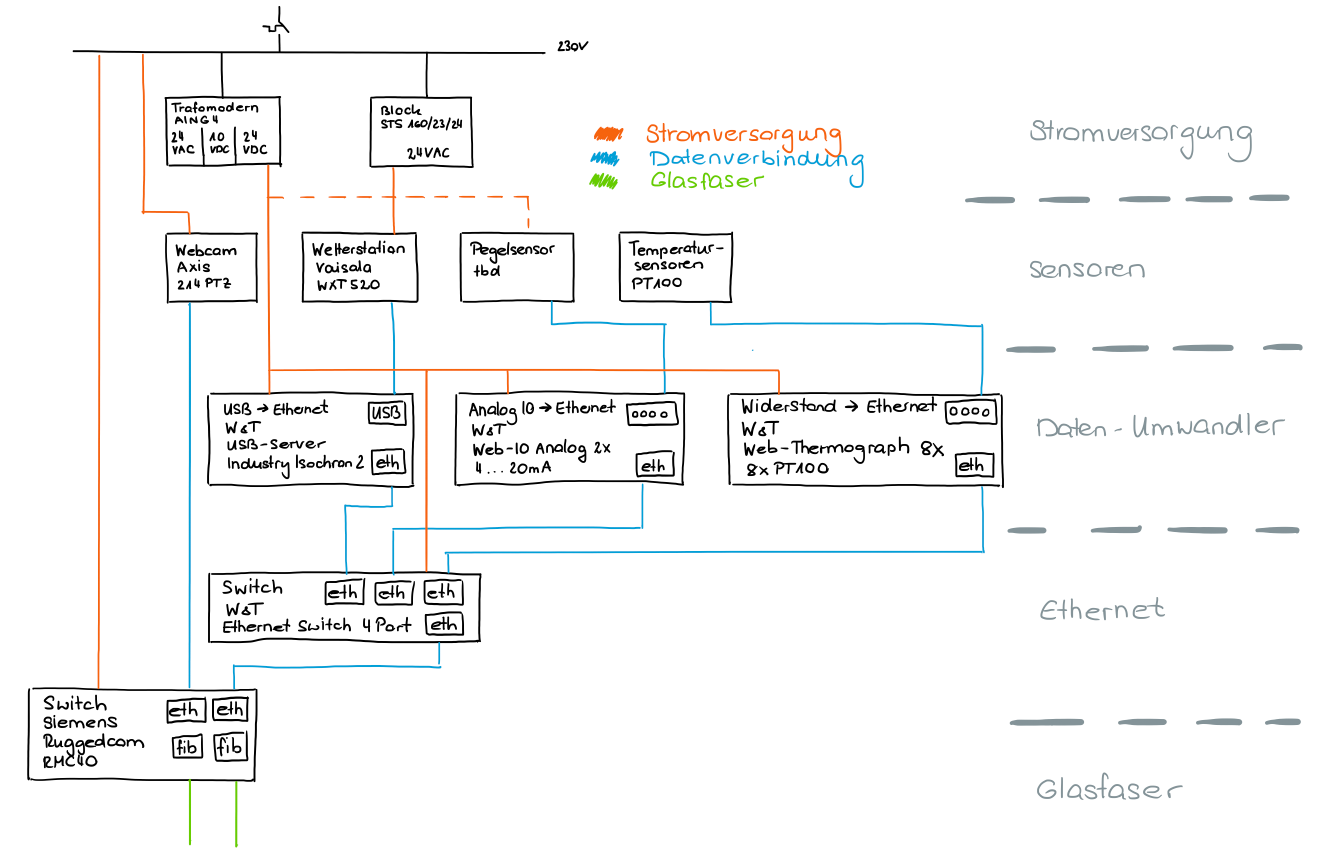
\includegraphics[width=1\linewidth]{img/HW-Aufbau}
	\caption{Hardware-Aufbau der Wetterstation Arbon}
	\label{img:HW-Aufbau}
\end{figure}



\section{Problemanalyse}
\Diskussionspunkt{Beschreibung, 
Begründung, 
Erkenntnisse aus IST-Analyse}

\subsection{Hardware}
Sowohl die Webcam, als auch der Kombi-Wetter-Transmitter funktionieren einwandfrei. Der defekte Temperaturwiderstand wird akzeptiert, da dessen Wert interpoliert werden kann. Der Pegel-Sensor hingegen ist defekt und muss ersetzt werden. Der bisherige Sensor nutzte das Prinzip der hydrostatischen Druckmessung. Für die Pegelmessung konnten wir drei verschiedene Messprinzipien eruiert, die eingesetzt werden können:

\begin{itemize}  
\item Hydrostatische Druckmessung
\item Ultraschall-Distanzmessung
\item Radar-Distanzmessung
\item Time-of-light-Distanzmessung
\end{itemize}




\section{SOLL-Zustand}
\Diskussionspunkt{Lösungsansätze = zu entwickelnde Artefakte, 
Resultat aus Literaturrecherche, 
Konzepte}





